% ============================================================================
%  Chapitre 5 : Estimation des moments d'inertie
% ============================================================================
\chapter{Estimation des moments d'inertie}


% ============================================================================
%  Chapitre 5, partie I : Position du problème
% ============================================================================

% ----------------------------------------------------------------------------
\section{Position du problème}
% ----------------------------------------------------------------------------

La simulation suppose connus la masse $m$, le rayon $a$ et la matrice
d'inertie $\mat{I}_b$ de la boule. Pour une vraie boule, $m$ et $a$ se
mesurent directement, avec une balance et un pied à coulisse. Ce n'est
pas le cas de $\mat{I}_b$, qui dépend de la répartition de la masse à
l'intérieur, ce que l'on ne connaît pas lors de la production. Le but de ce chapitre est de répondre à la question : "Comment peut-on les déterminer à partir de mesures embarquées ?". Dans ce chapitre, on utilise un gyromètre au centre de la boule, et éventuellement un accéléromètre.

\subsection{Le repère du gyromètre}

Dans les chapitres précédents, on a écrit l'inertie dans les axes
principaux de la boule, où $\mat{I}_b = \mathrm{diag}(I_1, I_2, I_3)$.
\textbf{Cependat, on ne connaît jamais ces axes}, et on ne peut donc pas y aligner le gyromètre. On doit travailler alors dans le repère du gyromètre, relié aux axes principaux par une rotation $\mat{P}$ inconnue. Dans ce repère, la matrice d'inertie
\[
    \mat{J} = \mat{P}\,\mat{I}_b\,\mat{P}^T
    = \begin{pmatrix}
        J_{11} & J_{12} & J_{13}\\
        J_{12} & J_{22} & J_{23}\\
        J_{13} & J_{23} & J_{33}
    \end{pmatrix}
\]
qui n'est plus diagonale, mais reste symétrique définie positive par définition. Estimer l'inertie revient donc à estimer ses $6$ coefficients, on ne peut pas faire autrement sans connaître $\mat{P}$.

\subsection{Retour aux axes principaux}

Une fois $\mat{J}$ estimée, on la diagonalise. Elle est symétrique,
donc
\[
    \mat{J} = \mat{P}\,\mathrm{diag}(I_1, I_2, I_3)\,\mat{P}^T,
    \qquad \mat{P} \in \SO
\]
Les valeurs propres de $\mat{J}$ sont les moments principaux
$I_1, I_2, I_3$, et les colonnes de $\mat{P}$ donnent les axes
principaux exprimés dans le repère du gyromètre. Donc, en plus, en diagonalisant $\mat{P}$, on obtient aussi la position du gyromètre par rapport aux axes principaux de l'inertie.


  \textbf{} % I. Position du probleme
\textbf{}
% ============================================================================
%  Chapitre 5, partie II : Les mesures
% ============================================================================

% ----------------------------------------------------------------------------
\section{Les mesures}
% ----------------------------------------------------------------------------

\subsection{Le gyromètre}

Le gyromètre que l'on va utiliser est le fameux \textbf{MPU6050} de protocol I2C, 
avec un bon timing et une bonne programmation, on peut avoir une fréquence de mesure de $ f=100 $ Hz.

Le gyromètre mesure la vitesse angulaire $\vect{\omega}$ de la boule
dans son propre repère, à la fréquence $f$, donc aux instants
$t_k = k/f$. Une mesure contient un
biais $\vect{b}$, que l'on suppose constant sur la durée d'une
expérience, et un bruit blanc gaussien $\vect{\nu}_k$ :
\[
    \vect{z}_k = \vect{\omega}(t_k) + \vect{b} + \vect{\nu}_k,
    \qquad
    \vect{\nu}_k \sim \mathcal{N}(0, \sigma^2\Id)
\]

\subsection{La verticale vue par la boule}
Les quantités conservées vont intervenir dans l'estimation, et pour $\vect{L} _G \vect{e}_z $, on a besoin de la matrice de changement de repère $\mat{R}$, donc éventuellement un magnétomètre si jamais on a besoin d'orientation de la sphère. Cependant, en supposant que l'on a très peu de bruit sur le gyromètre, une intégration sera suffisante pour réduire l'instalation d'un capteur. En effet, on a 
\[\vect{L}_G \vect{e}_z = \vect{e}_z ^T (\mat{R} \mat{I}_b \mat{R}^T \vect{\Omega}) = \vect{e}_z ^T \mat{R} \mat{I}_b \mat{R}^T \mat{R} \vect{\omega} = (\vect{e}_z ^T\mat{R})(\mat{I}_b \vect{\omega})
\]
Or
\[
    \vect{\gamma} = \mat{R}^T\vect{e}_z
\]
soit
\[
\vect{L}_G \vect{e}_z = \vect{\gamma} ^ T(\mat{I}_b \vect{\omega})
\]
\textbf{Évolution de $\vect{\gamma}$ : } on part de
$\dot{\mat{R}} = \mat{R}\hatx{\vect{\omega}}$. En transposant, et
comme $\hatx{\vect{\omega}}$ est antisymétrique,
\[
    \dot{\mat{R}}^T = \hatx{\vect{\omega}}^T\mat{R}^T
    = -\hatx{\vect{\omega}}\mat{R}^T
\]
Or $\vect{e}_z$ est fixe, donc
\[
    \dot{\vect{\gamma}} = \dot{\mat{R}}^T\vect{e}_z
    = -\hatx{\vect{\omega}}\vect{\gamma}
    = -\vect{\omega}\wedge\vect{\gamma}
\]
soit
\[
    \dot{\vect{\gamma}} = \vect{\gamma}\wedge\vect{\omega}
\]
\textbf{Intégration : } cette équation ne fait intervenir que
$\vect{\omega}$, que mesure le gyromètre. On peut donc obtenir
$\vect{\gamma}$ en l'intégrant à partir d'une valeur initiale
$\vect{\gamma}_0$. Celle-ci est donnée par l'accéléromètre (aussi sur le MPU6050), la boule
étant au repos, il mesure alors $g\,\vect{\gamma}_0$. Entre deux
mesures, on fait la rotation exacte par la vitesse angulaire moyenne
$\bar{\vect{\omega}}_k = \frac12(\vect{z}_k + \vect{z}_{k+1})$ :
\[
    \vect{\gamma}_{k+1}
    = \exp\bigl(-\Delta t\,\hatx{\bar{\vect{\omega}}_k}\bigr)\,\vect{\gamma}_k,
    \qquad \Delta t = 1/f
\]
où l'exponentielle se calcule par la formule de Rodrigues. Une rotation
conserve la norme : on garde $\|\vect{\gamma}_k\| = 1$ sans
renormaliser.

\textbf{Formule de Rodrigues : } pour $\vect{v} \in \R^3$ non nul, on
note $\phi = \|\vect{v}\|$ et $\vect{n} = \vect{v}/\phi$. Comme
$\hatx{\vect{n}}^3 = -\hatx{\vect{n}}$, la série de l'exponentielle se
regroupe en
\[
    \exp\bigl(\hatx{\vect{v}}\bigr)
    = \Id + \sin\phi\,\hatx{\vect{n}} + (1 - \cos\phi)\,\hatx{\vect{n}}^2
\]
c'est la rotation d'angle $\phi$ autour de $\vect{n}$. Ici,
$\vect{v} = -\Delta t\,\bar{\vect{\omega}}_k$ : avec
$\phi_k = \Delta t\,\|\bar{\vect{\omega}}_k\|$ et
$\vect{n}_k = \bar{\vect{\omega}}_k/\|\bar{\vect{\omega}}_k\|$, et
$\hatx{\vect{n}}^2\vect{x} = (\vect{n}\cdot\vect{x})\,\vect{n} - \vect{x}$,
\[
    \vect{\gamma}_{k+1} = \cos\phi_k\,\vect{\gamma}_k
    - \sin\phi_k\,\vect{n}_k\wedge\vect{\gamma}_k
    + (1 - \cos\phi_k)(\vect{n}_k\cdot\vect{\gamma}_k)\,\vect{n}_k
\]

\begin{remarque}[Traitement des données hors ligne]
    $\vect{\gamma}$ est obtenu en intégrant toutes les mesures du
    gyromètre depuis $t_0$, et son erreur grandit avec le temps. On
    traite donc les données hors ligne plutôt qu'en ligne.
\end{remarque}   % II. Les mesures

% ============================================================================
%  Chapitre 5, partie III : Mise en équation linéaire
% ============================================================================

% ----------------------------------------------------------------------------
\section{La mise en équations linéaires des contrôles}
% ----------------------------------------------------------------------------

On écrit maintenant les deux contrôles du modèle,
$\vect{L}_G\cdot\vect{e}_z$ et $T$, avec les seules mesures
$\vect{\omega}$ et $\vect{\gamma}$. Dans le repère du gyromètre,
$\mat{I}_b$ est remplacée par $\mat{J}$, et les deux contrôles
deviennent linéaires en ses coefficients.

\subsection{Moment cinétique vertical}

D'après la partie précédente, avec $\mat{J}$ à la place de
$\mat{I}_b$, dans le repère gyromètre
\[
    \vect{L}_G\cdot\vect{e}_z = \vect{\gamma}^T\mat{J}\,\vect{\omega} = c
\]
où $c$ est une constante inconnue. $\mat{J}$ n'est pas diagonale,
mais elle est symétrique donc 
\[
    J_{11}\gamma_1\omega_1 + J_{22}\gamma_2\omega_2 + J_{33}\gamma_3\omega_3
    + J_{12}(\gamma_1\omega_2 + \gamma_2\omega_1)
    + J_{23}(\gamma_2\omega_3 + \gamma_3\omega_2)
    + J_{13}(\gamma_1\omega_3 + \gamma_3\omega_1) - c = 0
\]

\subsection{Énergie cinétique}

\textbf{Vitesse du centre : } la boule roule sans glisser, donc
$\vect{v}_P = 0$, et $\overrightarrow{PG} = a\,\vect{e}_z$ donne
\[
    \vect{v}_G = \vect{v}_P + \vect{\Omega}\wedge\overrightarrow{PG}
    = a\,\vect{\Omega}\wedge\vect{e}_z
\]
Avec $\vect{\Omega} = \mat{R}\vect{\omega}$ et
$\vect{e}_z = \mat{R}\vect{\gamma}$, on a 
\[
    \vect{v}_G = a\,(\mat{R}\vect{\omega})\wedge(\mat{R}\vect{\gamma})
    = a\,\mat{R}\,(\vect{\omega}\wedge\vect{\gamma})
\]
Or $\mat{R}^T\mat{R} = \Id$, donc
\[
    \|\vect{v}_G\|^2 = a^2\|\vect{\omega}\wedge\vect{\gamma}\|^2
\]
et la relation
$\|\vect{u}\wedge\vect{v}\|^2 = \|\vect{u}\|^2\|\vect{v}\|^2 - (\vect{u}\cdot\vect{v})^2$,
avec $\|\vect{\gamma}\| = 1$, donne
\[
    \|\vect{v}_G\|^2 = a^2\bigl(\|\vect{\omega}\|^2 - (\vect{\gamma}^T\vect{\omega})^2\bigr)
\]

\textbf{Énergie : } l'énergie cinétique, conservée, s'écrit alors
\[
    2T = m\|\vect{v}_G\|^2 + \vect{\omega}^T\mat{J}\,\vect{\omega}
    = m a^2\bigl(\|\vect{\omega}\|^2 - (\vect{\gamma}^T\vect{\omega})^2\bigr)
    + \vect{\omega}^T\mat{J}\,\vect{\omega}
\]
En développant $\vect{\omega}^T\mat{J}\,\vect{\omega}$ et en passant
le terme connu à droite,
\[
    J_{11}\omega_1^2 + J_{22}\omega_2^2 + J_{33}\omega_3^2
    + 2J_{12}\omega_1\omega_2 + 2J_{23}\omega_2\omega_3
    + 2J_{13}\omega_1\omega_3 - 2T
    = -m a^2\bigl(\|\vect{\omega}\|^2 - (\vect{\gamma}^T\vect{\omega})^2\bigr)
\]

\subsection{Vecteur des paramètres}

Les deux équations sont linéaires en
\[
    \vect{\theta} = \begin{pmatrix}
        J_{11} & J_{22} & J_{33} & J_{12} & J_{23} & J_{13} & c & T
    \end{pmatrix}^T \in \R^8
\]
où les constantes $c$ et $T$, inconnues, sont estimées en même temps
que $\mat{J}$. Pour chaque mesure, on a donc
\[
    \vect{\varphi}_1(\vect{\gamma}, \vect{\omega})^T\vect{\theta} = 0,
    \qquad
    \vect{\varphi}_2(\vect{\gamma}, \vect{\omega})^T\vect{\theta} = y_2(\vect{\gamma}, \vect{\omega})
\]
avec
\begin{align*}
    \vect{\varphi}_1 &= \bigl(\gamma_1\omega_1,\ \gamma_2\omega_2,\
        \gamma_3\omega_3,\ \gamma_1\omega_2 + \gamma_2\omega_1,\
        \gamma_2\omega_3 + \gamma_3\omega_2,\
        \gamma_1\omega_3 + \gamma_3\omega_1,\ -1,\ 0\bigr)^T\\
    \vect{\varphi}_2 &= \bigl(\omega_1^2,\ \omega_2^2,\ \omega_3^2,\
        2\omega_1\omega_2,\ 2\omega_2\omega_3,\ 2\omega_1\omega_3,\
        0,\ -2\bigr)^T\\
    y_2 &= -m a^2\bigl(\|\vect{\omega}\|^2 - (\vect{\gamma}^T\vect{\omega})^2\bigr)
\end{align*}
   % III. Mise en equation lineaire

% ============================================================================
%  Chapitre 5, partie IV : Estimation par moindres carrés
% ============================================================================

% ----------------------------------------------------------------------------
\section{Estimation par moindres carrés}
% ----------------------------------------------------------------------------

\subsection{Modèle}

Pour la mesure $k$, on empile les deux équations de la partie
précédente :
\[
    \mat{\Phi}_k\,\vect{\theta} = \vect{y}_k,
    \qquad
    \mat{\Phi}_k = \begin{pmatrix}
        \vect{\varphi}_1(\vect{\gamma}_k, \vect{\omega}_k)^T\\
        \vect{\varphi}_2(\vect{\gamma}_k, \vect{\omega}_k)^T
    \end{pmatrix} \in \R^{2\times 8},
    \qquad
    \vect{y}_k = \begin{pmatrix} 0\\ y_2(\vect{\gamma}_k, \vect{\omega}_k)\end{pmatrix}
\]
Sur les $n$ mesures, on empile à nouveau les $\mat{\Phi}_k$ et les
$\vect{y}_k$ en $\mat{\Phi} \in \R^{2n\times 8}$ et
$\vect{y} \in \R^{2n}$ :
\[
    \mat{\Phi}\,\vect{\theta} = \vect{y}
\]

\subsection{Fonction de perte}

On cherche donc le $\vect{\theta}$ qui minimise l'erreur quadratique
sur toutes les mesures
\[
    \mathcal{L}(\vect{\theta})
    = \sum_{k=1}^{n}\frac12\|\vect{y}_k - \mat{\Phi}_k\vect{\theta}\|^2
    = \frac12\|\vect{y} - \mat{\Phi}\vect{\theta}\|^2
\]
Son gradient vaut
\[
    \nabla\mathcal{L}(\vect{\theta})
    = -\mat{\Phi}^T(\vect{y} - \mat{\Phi}\vect{\theta})
\]
et on obtient l'estimation de nos paramètres par : 
\[
    \mat{\Phi}^T\mat{\Phi}\,\vect{\theta} = \mat{\Phi}^T\vect{y}
    \quad\Longrightarrow\quad
    \hat{\vect{\theta}} = \bigl(\mat{\Phi}^T\mat{\Phi}\bigr)^{-1}\mat{\Phi}^T\vect{y}
\]

\subsection{Retour aux moments principaux}

De $\hat{\vect{\theta}}$, on reconstruit $\hat{\mat{J}}$, symétrique,
puis on la diagonalise comme dans la partie I :
\[
    \hat{\mat{J}} = \hat{\mat{P}}\,\mathrm{diag}(\hat{I}_1, \hat{I}_2, \hat{I}_3)\,\hat{\mat{P}}^T
\]
   % IV. Estimation par moindres carres

% ============================================================================
%  Chapitre 5, partie V : Validation sur des données synthétiques
% ============================================================================

% ----------------------------------------------------------------------------
\section{Validation sur des données synthétiques}
% ----------------------------------------------------------------------------

\subsection{Génération des données}

On simule la boule de référence ($m = 1$~kg, $a = 0{,}1$~m,
$\mat{I}_b = \mathrm{diag}(1{,}5;\ 8{,}5;\ 9{,}5)\cdot 10^{-3}$~kg$\cdot$m$^2$)
en quaternions pendant $5$~s, avec $h = 10^{-3}$~s. On en tire les
mesures d'un gyromètre à $f = 100$~Hz, soit $n = 501$ mesures, de
bruit $\sigma = 5\cdot 10^{-3}$~rad/s et de biais tiré selon
$\mathcal{N}(0, 10^{-6}\Id)$. Le gyromètre est monté dans la boule par
une rotation $\mat{Q}$ (repère du gyromètre vers axes principaux), et
mesure $\mat{Q}^T\vect{\omega}$. On note $\mat{J} = \mat{Q}^T\mat{I}_b\mat{Q}$
la matrice d'inertie vraie dans son repère.

On fait deux essais : un gyromètre aligné sur les axes principaux
($\mat{Q} = \Id$), puis un montage quelconque, où $\mat{Q}$ est tirée
uniformément sur $\SO$, à partir d'un quaternion unitaire uniforme.
Ces deux essais vérifient que la méthode fonctionne, sa précision
sera validée par une campagne de Monte-Carlo.

\subsection{Gyromètre aligné}

\begin{table}[H]
    \centering
    \begin{tabular}{lcc}
        \toprule
        Paramètre & Valeur vraie & Estimation \\
        \midrule
        $I_1$ ($10^{-3}$~kg$\cdot$m$^2$) & $1{,}500$ & $1{,}483$ \\
        $I_2$ ($10^{-3}$~kg$\cdot$m$^2$) & $8{,}500$ & $8{,}462$ \\
        $I_3$ ($10^{-3}$~kg$\cdot$m$^2$) & $9{,}500$ & $9{,}441$ \\
        $J_{12}, J_{23}, J_{13}$ ($10^{-3}$~kg$\cdot$m$^2$) & $0$ & $\le 0{,}02$ \\
        $c$ (kg$\cdot$m$^2$/s) & $0{,}0473$ & $0{,}0470$ \\
        $T$ (J) & $0{,}1349$ & $0{,}1342$ \\
        \bottomrule
    \end{tabular}
    \caption{Estimation avec un gyromètre aligné sur les axes principaux}
    \label{tab-estimation-aligne}
\end{table}

Les moments sont retrouvés à mieux que $1{,}2\,\%$, et les termes
croisés de $\hat{\mat{J}}$ sont bien quasi nuls.

\subsection{Montage quelconque}

Pour le montage tiré, la matrice d'inertie dans le repère du gyromètre
est pleine :
\[
    \mat{J} = \begin{pmatrix}
        7{,}078 & -2{,}653 & 1{,}281\\
        -2{,}653 & 4{,}890 & 2{,}886\\
        1{,}281 & 2{,}886 & 7{,}532
    \end{pmatrix}\cdot 10^{-3},
    \qquad
    \hat{\mat{J}} = \begin{pmatrix}
        7{,}030 & -2{,}601 & 1{,}256\\
        -2{,}601 & 4{,}868 & 2{,}854\\
        1{,}256 & 2{,}854 & 7{,}468
    \end{pmatrix}\cdot 10^{-3}
\]
En diagonalisant $\hat{\mat{J}}$ :

\begin{table}[H]
    \centering
    \begin{tabular}{lccc}
        \toprule
        & $I_1$ & $I_2$ & $I_3$ \\
        \midrule
        Valeur vraie ($10^{-3}$~kg$\cdot$m$^2$) & $1{,}500$ & $8{,}500$ & $9{,}500$ \\
        Estimation ($10^{-3}$~kg$\cdot$m$^2$) & $1{,}533$ & $8{,}417$ & $9{,}416$ \\
        Erreur relative & $2{,}2\,\%$ & $1{,}0\,\%$ & $0{,}9\,\%$ \\
        Erreur sur l'axe principal & $0{,}13^\circ$ & $0{,}27^\circ$ & $0{,}23^\circ$ \\
        \bottomrule
    \end{tabular}
    \caption{Estimation avec un montage quelconque du gyromètre}
    \label{tab-estimation-quelconque}
\end{table}
   % V. Validation sur des donnees synthetiques
% ============================================================================
%  Chapitre 5, partie VI : Campagne de Monte-Carlo
% ============================================================================

% ----------------------------------------------------------------------------
\section{Campagne de Monte-Carlo}
% ----------------------------------------------------------------------------

La partie précédente montre que notre estimation fonctionne sur les deux cas. On
veut maintenant savoir à quel point elle fonctionne en général, en la
lançant sur un grand nombre de scénarios tirés au hasard.

\subsection{Tirage des paramètres}

Un scénario est décrit par la variable aléatoire
\[
    X = (\vect{q}_0, \vect{\Omega}_0, m, a, \mat{I}_b, \mat{P})
\]
dont les composantes sont tirées indépendamment :
\begin{itemize}
    \item l'orientation initiale $\vect{q}_0$ et le montage $\mat{P}$
    sont uniformes sur $\SO$, tirés à partir d'un quaternion unitaire
    uniforme, plutôt que sur les intervalles qui définissent les angles d'Euler 
    pour éviter la concentration près des pôles. (Imaginons que l'on soit dans le cas d'un globle
    avec la longitude et la latitude, les lignes se concentrent aux pôles).
    \item $\vect{\Omega}_0$, $m$ et $a$ sont uniformes sur les
    intervalles du tableau~\ref{tab-lois-mc}.
    \item $\mat{I}_b = ma^2\,\mathrm{diag}(\lambda_1, \lambda_2, \lambda_3)$,
    où les moments propres $\lambda_i$ sont uniformes sur
    $[\lambda_{\min}, \lambda_{\max}]$.
\end{itemize}

Le gyromètre garde les réglages de la partie V : $f = 100$~Hz,
$\sigma = 5\cdot 10^{-3}$~rad/s, biais selon $\mathcal{N}(0, 10^{-6}\Id)$,
et $5$~s de mesure. Certes, dans la réalité, le biais a des drifts, et la fréquence de capteur n'est pas tout le temps $100\%$ à cause des bruits ou de mauvais timing dans le code. Pour ce niveau de validation, je le garderai pour la validation finale.

\begin{table}[H]
    \centering
    \begin{tabular}{lcc}
        \toprule
        Paramètre & Loi & Intervalle \\
        \midrule
        $\vect{q}_0$, $\mat{P}$ & uniforme sur $\SO$ & \\
        $\Omega_{0,x}$, $\Omega_{0,y}$ (rad/s) & uniforme & $[-2;\ 2]$ \\
        $\Omega_{0,z}$ (rad/s) & uniforme & $[-6;\ 6]$ \\
        $m$ (kg) & uniforme & $[0{,}5;\ 2]$ \\
        $a$ (m) & uniforme & $[0{,}05;\ 0{,}15]$ \\
        $\lambda_1, \lambda_2, \lambda_3$ & uniforme & $[0{,}1;\ 1]$ \\
        \bottomrule
    \end{tabular}
    \caption{Lois des paramètres de la campagne de Monte-Carlo}
    \label{tab-lois-mc}
\end{table}
\textbf{Validation du scénario : } le résultat d'un scénario n'est gardé que s'il est
physique et exploitable :
\begin{itemize}
    \item inégalités d'inertie : $\lambda_1 + \lambda_2 \ge \lambda_3$ (et
    permutations).

    \item masse dans la boule : $\lambda_1 + \lambda_2 + \lambda_3 \le 2$,
    car $I_1 + I_2 + I_3 = 2\int \|\vect{x}\|^2\,\mathrm{d}m \le 2ma^2$.
    \item mouvement assez excité : $\|\vect{\Omega}_0\| \ge \Omega_{\min}$,
    sinon rien ne se passera.
    \item non-glissement vérifié sur toute la simulation : $|N| \le \mu_s m g$.
\end{itemize}
Sinon, on retire le scénario. $X$ suit donc la loi uniforme conditionnée
à l'ensemble des scénarios admissibles.

\subsection{Critères et Estimation de la Performance de la méthode}

\textbf{Erreur relative de moment d'inertie d'un scénario : } pour le scénario $X_k$, la simulation
donne la vraie matrice $\mat{J}_k = \mat{P}_k\mat{I}_{b,k}\mat{P}_k^T$, et
l'estimation donne $\hat{\mat{J}}_k$. On définit l'erreur relative d'inertie
\[
    \varepsilon_k = \frac{\|\hat{\mat{J}}_k - \mat{J}_k\|_F}{\|\mat{J}_k\|_F}
\]

\textbf{Variable de succès de la méthode pour un scénario : } pour une tolérance $\mathrm{tol_{est}}$ fixée,
on pose
\[
    S_k = \mathbf{1}_{\{\varepsilon_k < \mathrm{tol_{est}}\}}
\]
Les scénarios sont indépendants et de même loi, donc les $S_k$ sont des
variables de Bernoulli indépendantes de paramètre
\[
    p = \mathbb{P}(\varepsilon < \mathrm{tol_{est}}) = \mathbb{E}[S_k]
\]
le taux de réussite de la méthode, ce qui décrit la performance. Le nombre de succès sur $N$
scénarios suit alors la loi binomiale $\mathcal{B}(N, p)$.

\textbf{Estimation de $p$ : } on estime $p$ par la proportion de
succès
\[
    \hat{p}_N = \frac{1}{N}\sum_{k=1}^{N} S_k
\]
qui est sans biais, $\mathbb{E}[\hat{p}_N] = p$, de variance
$p(1-p)/N$, et qui converge presque sûrement vers $p$ par la LFGN. Par le théorème central limite, un intervalle de
confiance à $95\,\%$ est
\[
    \hat{p}_N \pm 1{,}96\sqrt{\frac{\hat{p}_N(1-\hat{p}_N)}{N}}
\]
\subsection{Résultat}

On lance la campagne sur $N = 3000$ scénarios admissibles. Aucune
estimation n'échoue, et $\mat{\Phi}^T\mat{\Phi}$ est toujours inversible.

\begin{figure}[H]
    \centering
    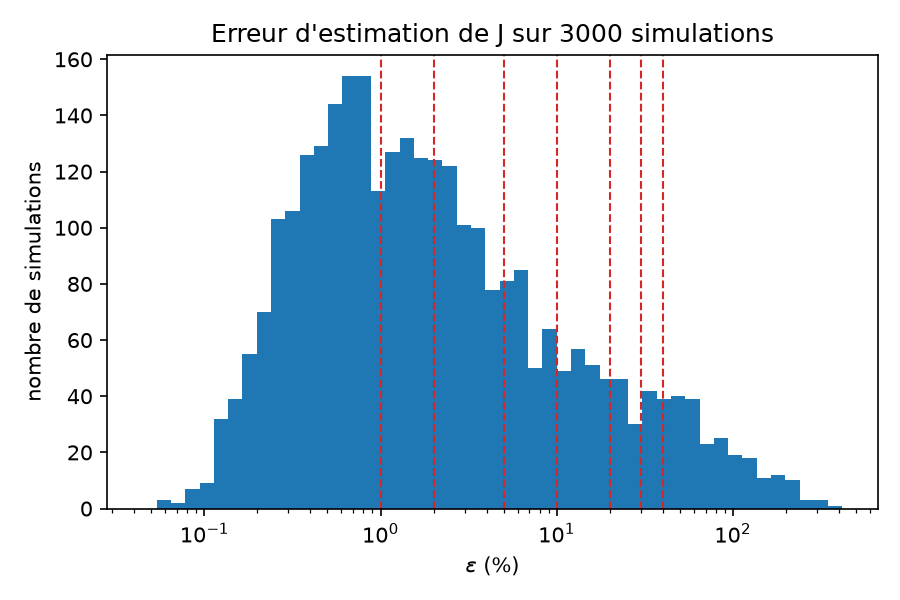
\includegraphics[width=0.75\textwidth]{chapitre5/figures/hist_eps.png}
    \caption{Distribution de l'erreur $\varepsilon$ sur les $3000$
    scénarios (échelle logarithmique), les pointillés sont les
    tolérances du tableau~\ref{tab-taux-mc}}
    \label{fig-hist-eps}
\end{figure}
\begin{figure}[H]
    \centering
    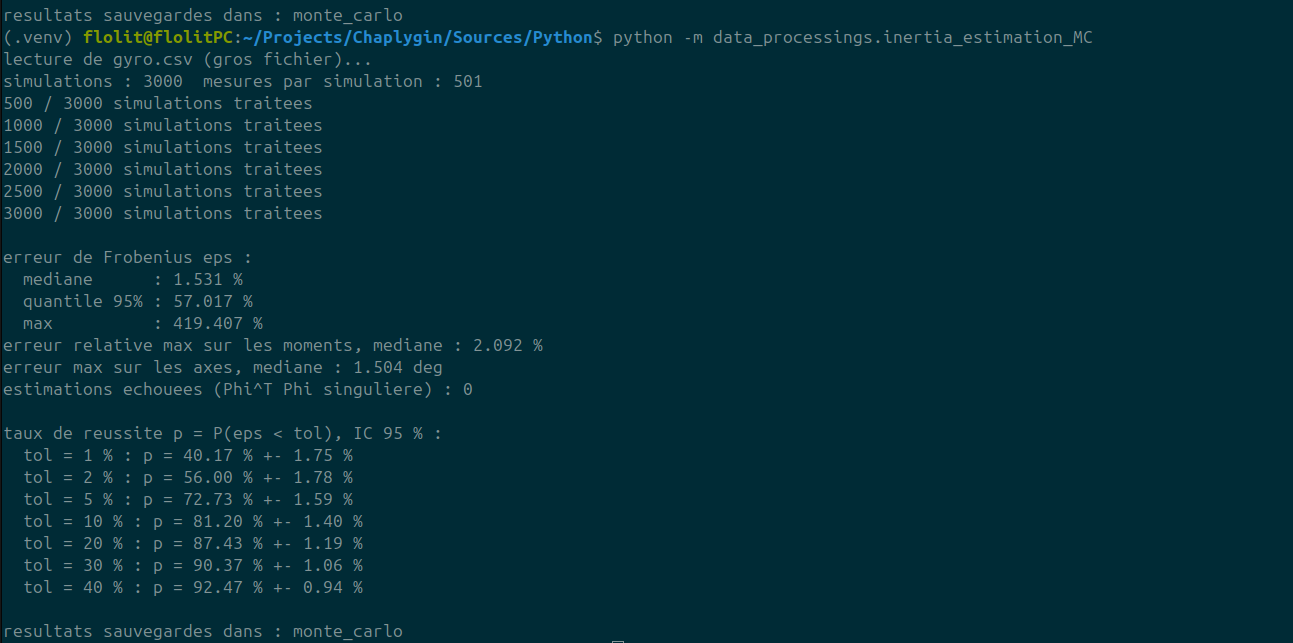
\includegraphics[width=0.75\textwidth]{chapitre5/figures/Result_3000sims.png}
    \caption{Résultats des $3000$ simulations}
    \label{fig-terminal}
\end{figure}
\newpage
Voici le résultat du traitement de données de la simulation Monte-Carlo.
\begin{table}[H]
    \centering
    \begin{tabular}{cc}
        \toprule
        $\mathrm{tol_{est}}$ & $\hat{p}_N$ (IC $95\,\%$) \\
        \midrule
        $1\,\%$  & $40{,}2 \pm 1{,}8\,\%$ \\
        $2\,\%$  & $56{,}0 \pm 1{,}8\,\%$ \\
        $5\,\%$  & $72{,}7 \pm 1{,}6\,\%$ \\
        $10\,\%$ & $81{,}2 \pm 1{,}4\,\%$ \\
        $20\,\%$ & $87{,}4 \pm 1{,}2\,\%$ \\
        $30\,\%$ & $90{,}4 \pm 1{,}1\,\%$ \\
        $40\,\%$ & $92{,}5 \pm 0{,}9\,\%$ \\
        \bottomrule
    \end{tabular}
    \caption{Taux de réussite estimé selon la tolérance}
    \label{tab-taux-mc}
\end{table}

\textbf{Commentaires : }
\begin{itemize}
    \item Pour un scénario typique, la méthode marche bien : l'erreur
    médiane est près de $\varepsilon = 1{,}5\,\%$.
    \item La distribution a pourtant une longue queue : $\approx 10\,\%$ des
    scénarios ont une erreur au-delà de $30\,\%$.
\end{itemize}
\begin{proposition}[Ce qu'il faudra faire]
    Jusqu'à ce stade, l'idée de l'algorithme est validée, on a une estimation suffisamment satisfaisante. Afin d'avoir une meilleure performance, il nous faut alors étudier les grosses erreurs et leurs causes.
\end{proposition}

 % VI. Design de la campagne de validation MC